\newpage
\section*{Модели отражения} 

Радиоволна, как и любая другая электромагнитная волна, отражается от препятствий, причем препятствием является любая неоднородность электрических или магнитных параметров среды, то есть объект отражает электромагнитную энергию, в случае если проводимость, диэлектрическая или магнитная проницаемость отличается от соответствующих параметров среды.
Так как от поверхности в результате процесса отражения отходит электромагнитная энергия, то можно считать, что отражатель сам является источником (вторичным) электромагнитного излучения. Это явление можно также представить себе следующим образом: при попадании волны на поверхность предмета, она в нем порождает вынужденные колебания зарядов, которые синхронны с колебаниями падающей волны. Колебания зарядов создают токи смещения и токи проводимости, и сами становятся источниками излучения. Каждый такой элементарный ток в рамках достаточного малого точечного объема можно считать источником новой сферической волны. Общий результат таких элементарных токов (в соответствии с принципом Гюйгенса-Френеля \cite{gugens}) суммируется с различными фазовыми соотношениями и может принимать разные значения, а падающая волна отражается во всех направлениях. Значит, энергия переизлучается в различных направлениях неравномерно \cite{radiolocation}.

Радиоволны и световые волны имеют одну и ту же физическую электромагнитную природу, поэтому многие модели поведения света известные из оптики (кстати как и способы получения фотореалистических изображений компьютерной геометрии) применимы в нашем случае. Рассмотрим основные модели отражения радиоволн: зеркальное, диффузное и резонансное. Подробнее информацию об этом можно найти в \cite{radiolocation}.

\subsection*{Зеркальное отражение}

Условие возникновения: линейные размеры отражающей поверхности много больше длины волны ($ l >> \lambda $), а сама поверхность является достаточно гладкой ($ h << \lambda $), где $ l $ -- наименьшией линейный размер цели; $ \lambda $ -- длина волны; $ h $ -- высота неровностей поверхности. 

Свойства зеркального отражения известны еще с давних времен и являются следствиями применения принципа Ферма к отражающей поверхности \cite{ferma}:

- луч отраженный, луч падающей, а также нормаль отражающей поверхности, проведенная к точке падения, лежат в одной плоскости;

- угол падения равен углу отражения.

\begin{center}
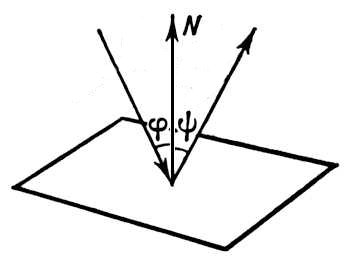
\includegraphics[width=0.25\linewidth]{zerkalo.jpg}
\end{center}

Интенсивность отражённого света характеризуется коэффициентом отражения и зависит от соотношения показателей преломления сред, от угла падения и поляризации падающего пучка лучей. Количественно эту зависимость выражают формулы Френеля \cite{frenel}.

\subsection*{Диффузное отражение}

Условие возникновения: линейные размеры отражающей поверхности много больше длины волны ($ l >> \lambda $), а неровности поверхности имеют порядок длины волны (или больше) и расположены хаотично, то есть поверхность является шераховатой (матовой) ($ h \ge \lambda $). 

При диффузном отражении энергия рассеивается во всех направлениях. Для матовых поверхностей применимы законы Ламберта \cite{lambert}: для потока излучения, падающего нормально к матовой поверхности, мощность вторичного излучения под углом $ \gamma $ к нормали пропорциональна $ cos \gamma $. 
\begin{gather}
 P = P_0 \cdot cos \gamma
\end {gather}

\begin{center}
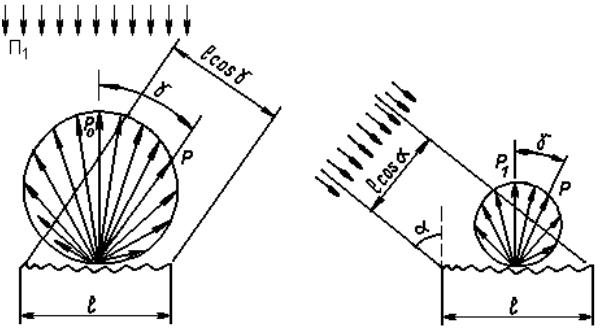
\includegraphics[width=0.6\linewidth]{lambert.jpg}
\end{center}

Если поток излучения падает под углом $\alpha$ к поверхности, то 
\begin{gather}
 P = P_0 \cdot cos \alpha \cdot cos \gamma
\end {gather}
где $ P_0 $ -- мощность, которую принимал бы приемник, если бы облучение шло с "зенита", то есть с увеличением $\alpha$ уменьшается перехватываемый поверхностью падающий поток, отчего уменьшается освещенность и яркость. 

Условия зеркальности и диффузно отражающих поверхностей являются расплывчатыми. Здесь \cite{radiolocation} дается строгая формулировка и вывод критерия различия зеркальных и матовых поверхностей. Скажем лишь, что тип поверхностей зависит сразу от трех факторов: высоты неровностей поверхности $h$, длины волны $\lambda$ и угла падения $\phi$.

Закон Ламберта -- закон идеального рассеивания света, то есть это некоторая модель, к которой можно приблизиться, но которой не существует в естественных условиях. В реальной жизни поверхности обычно дают отражение, представляемое смесью диффузной и зеркальной состовляющих. 

\begin{center}
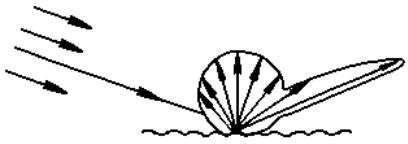
\includegraphics[width=0.45\linewidth]{diffuzerkalo.jpg}
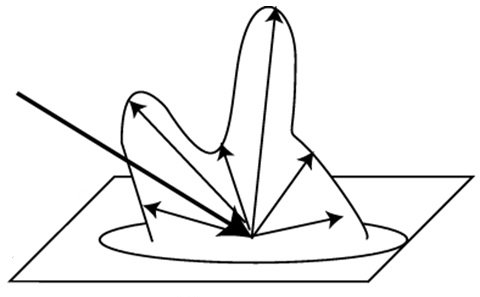
\includegraphics[width=0.45\linewidth]{glossy.jpg}
\end{center}

Кроме того, на практике, часто встречаются материалы имеющие несколько максимумов под разными углами и дающие в соответствующих направлениях из-за этого блеск (glossy materials).

Все вышеперечисленные свойства можно смоделировать воспользовавшись функцией, характеризующей степень отражения в данном направлении. Такая функция называется ДФО -- двулучевая функцией отражения (BRDF -- Bidirectional Reflection Distribution Function). Так для диффузных моделей ДФО равна константе. 

\begin{center}
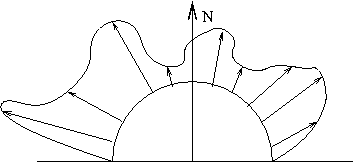
\includegraphics[width=0.45\linewidth]{dfo.png}
\end{center}

Именно эту функцию мы и будем использовать в нашей работе. Таким образом достигается некоторая универсальность -- наша программа сможет моделировать не только какой-то один конкретный вид отражения, а появляется возможность это задать в достаточно независимом виде. 

\subsection*{Резонансное отражение}

Список моделей отражения был бы не полон если не упомянуть резонансное отражение. Как уже было отмечено, падающая волна создает вынужденные колебания свободных или связанных зарядов в поверхности предмета. Тело, способное переизлучать электромагнитную волну, обладает собственной частотой колебаний частиц, несущих электрический заряд. Причем, если частота колебаний падающей волны совпадает с собственной частотой колебаний в поверхности, то имеем не что иное как явление резонансного отражения. В этом случае появляется ярко выраженная направленность вторичного излучения. Подробнее об этом явлении можно прочитать в \cite{radiolocation}.


